\documentclass[12pt, oneside]{article}
\usepackage[letterpaper, margin=1in]{geometry}
\usepackage[english]{babel}
\usepackage[utf8]{inputenc}
\usepackage{amsmath}
\usepackage{amsfonts}
\usepackage{amssymb}
\usepackage{tikz}
\usepackage{tkz-fct}

\usepackage{fancyhdr}
\pagestyle{fancy}
\fancyhf{}
\rhead{\thepage \\Name: \hspace{1.5in}.\\}
\lhead{BECA / Dr. Huson / 11.1 IB Math SL \\* 24 May 2018 \\* \textbf{Take home test: Functions, exponents, \& imaginary numbers}}

\vspace{1cm}

\renewcommand{\headrulewidth}{0pt}

\title{Problem set template}
\author{Chris Huson}
\date{May 2018}

\begin{document}
%\maketitle

\subsubsection*{\\* \textnormal{Open book \& open note. No searching online for answers. No electronic calculators (no Desmos), only handhelds.}}

\begin{enumerate}


\item Simplify the expression $(2 + 2i)^2$, where $i$ is the imaginary unit. \\*[.75in]

\item Write $\sqrt[3]{x^4} \bullet \sqrt[3]{x^2}$ as a single term with a rational or integer exponent.\\*[1in]

\item The polynomial $f(x)$ shown has a leading coefficient of 1. Write an equation for $f(x)$ in factored form.\\*[20pt]
\begin{center}
    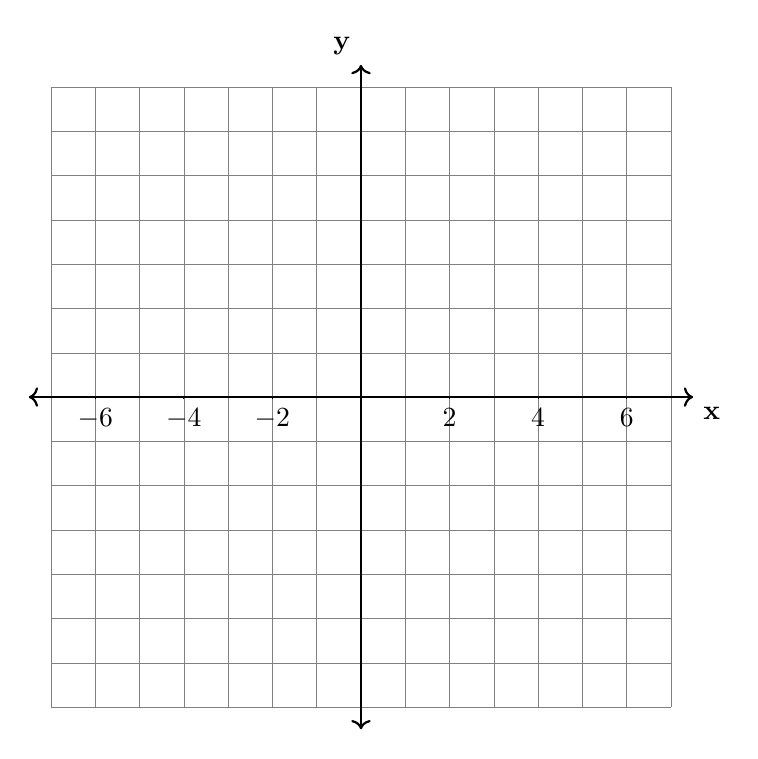
\begin{tikzpicture}[scale=2.25/4]
    \draw[step=1cm,gray,very thin] (-7,-7) grid (7,7);
    \draw[thick,<->] (-7.5,0) -- (7.5,0) node[anchor=north west] {\textbf{x}};
    \draw[thick,<->] (0,-7.5) -- (0,7.5) node[anchor=south east] {\textbf{y}};
    \foreach \x in {-6, -4, -2, 2, 4, 6} \draw (\x cm,1pt) -- (\x cm,-1pt) node[anchor=north] {$\x$};
    %\foreach \y in {5} \draw (1pt,\y cm) -- (-1pt,\y cm) node[anchor=east] {50}; %{$\y$};
    \tkzInit[xmin=-6,xmax=5,ymin=-7,ymax=7,ystep=1]   
    \tkzFct[color=black,thick,<->,domain = -4.3:4.9] {0.1*(x+3)*(x+1)*(x-4)};
    \end{tikzpicture}
\end{center}
The function $g$ is formed by translating function $f$ right 2 units. Sketch $y=g(x)$ on the same grid.

\newpage

\item Given: $f(x)=5x^2 - 2x + 1$ and $g(x)=x+1$\\*[5pt]
Express $f(x) \bullet g(x) + g(x)$ as a polynomial in standard form. \\*[3in]


\item When $x>0$ and $d$ is a positive integer, the expression $\displaystyle \left(9x \right)^\frac{d}{2}$ is equivalent to what expressed as a radical? \\*[2in]

\item What are the zeros for $f(x)=x^4+x^3-19x^2+11x+30$? (hint: graph it on the calculator) \\*[1in]  

\newpage

\item Sketch a graph of a cubic polynomial with the following characteristics: 
\begin{itemize}
\item three positive, real zeros
\item as $x \rightarrow + \infty$, $f(x) \rightarrow - \infty$
\item as $x \rightarrow - \infty$, $f(x) \rightarrow + \infty$
\end{itemize}
\begin{center}
    \begin{tikzpicture}[scale=2/4]
    \draw[thick,<->] (-7.5,0) -- (7.5,0) node[anchor=north west] {\textbf{x}};
    \draw[thick,<->] (0,-7.5) -- (0,7.5) node[anchor=south east] {\textbf{y}};
    \end{tikzpicture}
\end{center} %Alg2 Regents Jun2016 MC


\item Algebraically determine the values of $h$ and $k$ to correctly complete the identity stated below.
\[x^3+3x^2+5x+3=(x+1)(x^2+hx+k)\] %\\*[3in]

\newpage
\item The zeros of a cubic polynomial function $f$ are  $-5, 2, \text{ and } 5$. The polynomial has a negative leading coefficient, $a<0$. Sketch a graph of $y = f(x)$ on the grid below.\\*
\begin{center}
    
\begin{tikzpicture}
    \draw[step=0.25in,gray,very thin] (0,0) grid (12.7,12.7);
    \end{tikzpicture}
\end{center}
Write an equation for $f(x)$ in factored form, assuming the leading coefficient is negative one.\\*[30pt]

\newpage

\item Explain how $\displaystyle \left( \frac{8}{y^3} \right)^\frac{2}{3}$ is equivalent to $\displaystyle \frac{4}{y^2}$. \\*[2.5in]


\item Given that the remainder when  $f(x)=2x^3+6x^2+5x+8$ is divided by $x+3$ is $-7$. What is the value of $f(-3)$? \\*[1.5in]

\item Given $i$ is the imaginary unit, $(3-xi)^2$ in simplest form is what?  \\*[1.25in]


\newpage

\item For the polynomial with graph shown, state 
\begin{enumerate}
\item its degree \\[0.25in]
\item how many distinct zeros it has \\[0.25in]
\item the sign of its leading coefficient \\[0.25in]
\end{enumerate}

    \begin{tikzpicture}[scale=2/4]
    %\draw[step=1cm,gray,very thin] (-7,-7) grid (7,7);
    \draw[thick,<->] (-7.5,0) -- (7.5,0) node[anchor=north west] {\textbf{x}};
    \draw[thick,<->] (0,-7.5) -- (0,7.5) node[anchor=south east] {\textbf{y}};
    %\foreach \x in {-6, -4, -2, 2, 4, 6} \draw (\x cm,1pt) -- (\x cm,-1pt) node[anchor=north] {$\x$};
    %\foreach \y in {5} \draw (1pt,\y cm) -- (-1pt,\y cm) node[anchor=east] {50}; %{$\y$};
    \tkzInit[xmin=-6,xmax=6,ymin=-7,ymax=7,ystep=1]   
    \tkzFct[color=black,thick,<->,domain = -4.3:5.2] {-0.1*(x+3)*(x)*(x-4)};
    \end{tikzpicture}

\item Simplify the expression $\displaystyle \frac{5x^3+35x^2-10x}{5x}$, where $x \neq 0$.  \\*[1in]



\newpage

\item Given $N(t)=N_0(e)^{-rt}$, where $N(t)$ is the amount of a drug, $N_0$ is the initial dosage, $r$ is the decay rate, and $t$ is time in hours.\\[5pt] For $A$, model $A(t)$ as an initial amount of 190 milligrams and decay rate of 0.20.\\[5pt]
For $B, B(t)$ is 65 milligrams initially with a decay rate of 0.07.\\*[5pt]
Write equations for $A(t)$ and $B(t)$.\\[.75in]
Graph each function on the set of axes below.
\begin{center}
    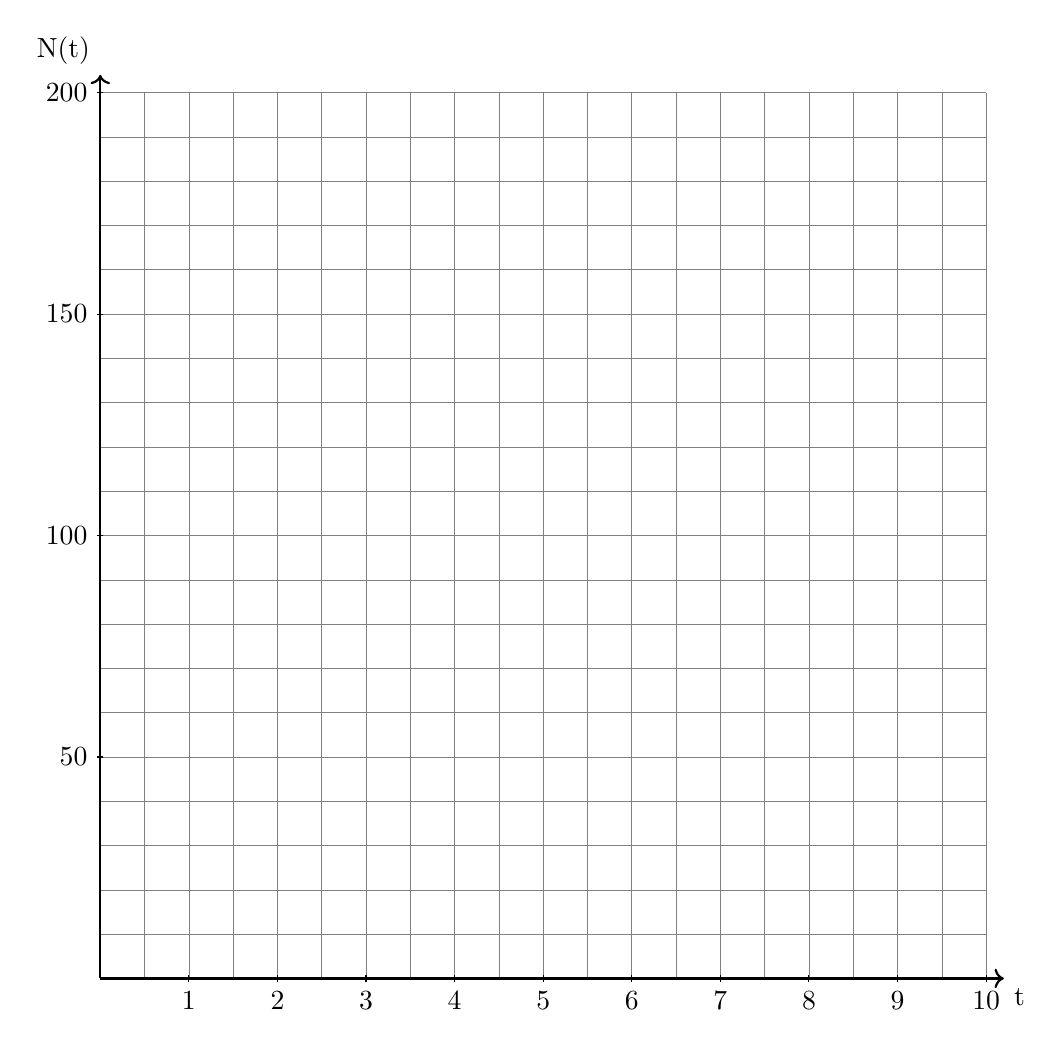
\begin{tikzpicture}[scale=4.5/4]
    \draw[step=0.5cm,gray,very thin] (0,0) grid (10,10);
    \draw[thick,->] (0,0) -- (10.2,0) node[anchor=north west] {t};
    \draw[thick,->] (0,0) -- (0,10.2) node[anchor=south east] {N(t)};
    \foreach \x in {1,2,3,4,5,6,7,8,9,10} \draw (\x cm,1pt) -- (\x cm,-1pt) node[anchor=north] {$\x$};
    \foreach \y in {2.5} \draw (1pt,\y cm) -- (-1pt,\y cm) node[anchor=east] {50};
    \foreach \y in {5} \draw (1pt,\y cm) -- (-1pt,\y cm) node[anchor=east] {100};
    \foreach \y in {7.5} \draw (1pt,\y cm) -- (-1pt,\y cm) node[anchor=east] {150};
    \foreach \y in {10} \draw (1pt,\y cm) -- (-1pt,\y cm) node[anchor=east] {200};
    \end{tikzpicture}
\end{center}
To the \emph{nearest hour}, $t$, when will the two drugs be at equal levels?\\*[0.5in]
When will $145$ milligrams of drug $A$ remain, to the \emph{nearest tenth of an hour}? 

\newpage


\item A suburban high school has a population of 1376 students. The number of students who participate in sports is 649. The number of students who participate in music is 433. If
the probability that a student participates in either sports or music is $\displaystyle \frac{974}{1376}$, what is the probability that a student participates in both sports and music?\\[2.75in] %Alg2 Regents Jun2016

\item If $g(c)=1-c^2$ and $m(c)=c+1$, then which statement is \emph{not} true?
\begin{enumerate}
    \item $g(c) \bullet m(c) = 1+c-c^2-c^3$
    \item $g(c) + m(c) = 2+c-c^2$
    \item $m(c) - g(c) = c+c^2$
    \item $\displaystyle \frac{m(c)}{g(c)} = \frac{-1}{1-c}$ \\[.75in]
\end{enumerate} %Regents Alg2 Jun2016

\item Sean’s team has a baseball game tomorrow. He pitches 50\% of the games. There is a 40\% chance of rain during the game tomorrow. If the probability that it rains given that Sean pitches is 40\%, it can be concluded that these two events are
\begin{enumerate}
    \item independent
    \item dependent
    \item mutually exclusive
    \item complements
\end{enumerate} %Regents Alg2 Jun2016


\newpage

\item Sketch a graph with the following characteristics: 
\begin{itemize}
\item polynomial function of order four
\item a positive leading coefficient
\item four real zeros
\end{itemize}
\begin{center}
    \begin{tikzpicture}[scale=2/4]
    \draw[thick,<->] (-7.5,0) -- (7.5,0) node[anchor=north west] {\textbf{x}};
    \draw[thick,<->] (0,-7.5) -- (0,7.5) node[anchor=south east] {\textbf{y}};
    \end{tikzpicture}
\end{center}

\newpage

\item For each polynomial graph, state 
\begin{enumerate}
\item its degree,
\item how many distinct zeros it has, and
\item the sign of its leading coefficient.
\end{enumerate}

    \begin{tikzpicture}[scale=2/4]
    %\draw[step=1cm,gray,very thin] (-7,-7) grid (7,7);
    \draw[thick,<->] (-7.5,0) -- (7.5,0) node[anchor=north west] {\textbf{x}};
    \draw[thick,<->] (0,-7.5) -- (0,7.5) node[anchor=south east] {\textbf{y}};
    %\foreach \x in {-6, -4, -2, 2, 4, 6} \draw (\x cm,1pt) -- (\x cm,-1pt) node[anchor=north] {$\x$};
    %\foreach \y in {5} \draw (1pt,\y cm) -- (-1pt,\y cm) node[anchor=east] {50}; %{$\y$};
    \tkzInit[xmin=-6,xmax=6,ymin=-7,ymax=7,ystep=1]   
    \tkzFct[color=black,thick,<->,domain = -4.3:5.2] {-0.1*(x+3)*(x)*(x-4)};
    \end{tikzpicture}
    \begin{tikzpicture}[scale=2/4]
    %\draw[step=1cm,gray,very thin] (-7,-7) grid (7,7);
    \draw[thick,<->] (-7.5,0) -- (7.5,0) node[anchor=north west] {\textbf{x}};
    \draw[thick,<->] (0,-7.5) -- (0,7.5) node[anchor=south east] {\textbf{y}};
    %\foreach \x in {-6, -4, -2, 2, 4, 6} \draw (\x cm,1pt) -- (\x cm,-1pt) node[anchor=north] {$\x$};
    %\foreach \y in {5} \draw (1pt,\y cm) -- (-1pt,\y cm) node[anchor=east] {50}; %{$\y$};
    \tkzInit[xmin=-6,xmax=6,ymin=-7,ymax=7,ystep=1]   
    \tkzFct[color=black,thick,<->,domain = -5.3:4.2] {-0.05*(x+5)*(x+3)*(x-1)*(x-4)};
    \end{tikzpicture}
\\[30pt]
    \begin{tikzpicture}[scale=2/4]
    %\draw[step=1cm,gray,very thin] (-7,-7) grid (7,7);
    \draw[thick,<->] (-7.5,0) -- (7.5,0) node[anchor=north west] {\textbf{x}};
    \draw[thick,<->] (0,-7.5) -- (0,7.5) node[anchor=south east] {\textbf{y}};
    %\foreach \x in {-6, -4, -2, 2, 4, 6} \draw (\x cm,1pt) -- (\x cm,-1pt) node[anchor=north] {$\x$};
    %\foreach \y in {5} \draw (1pt,\y cm) -- (-1pt,\y cm) node[anchor=east] {50}; %{$\y$};
    \tkzInit[xmin=-6,xmax=6,ymin=-7,ymax=7,ystep=1]   
    \tkzFct[color=black,thick,<->,domain = -1.3:5.2] {-0.5*(x-2)*(x-2)};
    \end{tikzpicture}
    \begin{tikzpicture}[scale=2/4]
    %\draw[step=1cm,gray,very thin] (-7,-7) grid (7,7);
    \draw[thick,<->] (-7.5,0) -- (7.5,0) node[anchor=north west] {\textbf{x}};
    \draw[thick,<->] (0,-7.5) -- (0,7.5) node[anchor=south east] {\textbf{y}};
    %\foreach \x in {-6, -4, -2, 2, 4, 6} \draw (\x cm,1pt) -- (\x cm,-1pt) node[anchor=north] {$\x$};
    %\foreach \y in {5} \draw (1pt,\y cm) -- (-1pt,\y cm) node[anchor=east] {50}; %{$\y$};
    \tkzInit[xmin=-6,xmax=6,ymin=-7,ymax=7,ystep=1]   
    \tkzFct[color=black,thick,<->,domain = -3.3:5.2] {0.05*(x*x*x*x-3*x*x*x-9*x*x+10*x+20)};
    \end{tikzpicture}


\newpage


\item What is the expression $6xi^3(-4xi+5)$ is equivalent to?  %Alg2 Regents Jun2017 multiple choice

\item Simplify the expression $(3k - 2i)^2$, where $i$ is the imaginary unit. %Alg2 Regents Aug2017




\newpage

\end{enumerate}
\end{document}
